\frame{
\begin{itemize}
	\item the observation of polarization phenomenon;

	\phantom{239}

	\item studing the methods of getting a polarized light;

	\phantom{239}

	\item looking at the aspects of polarization and some magic.
\end{itemize}	\frametitle{Our aims in this work}
}

\section{Mirror}

\frame{
\begin{minipage}{0.55\textwidth}
    \begin{figure}[h]
    \centering
    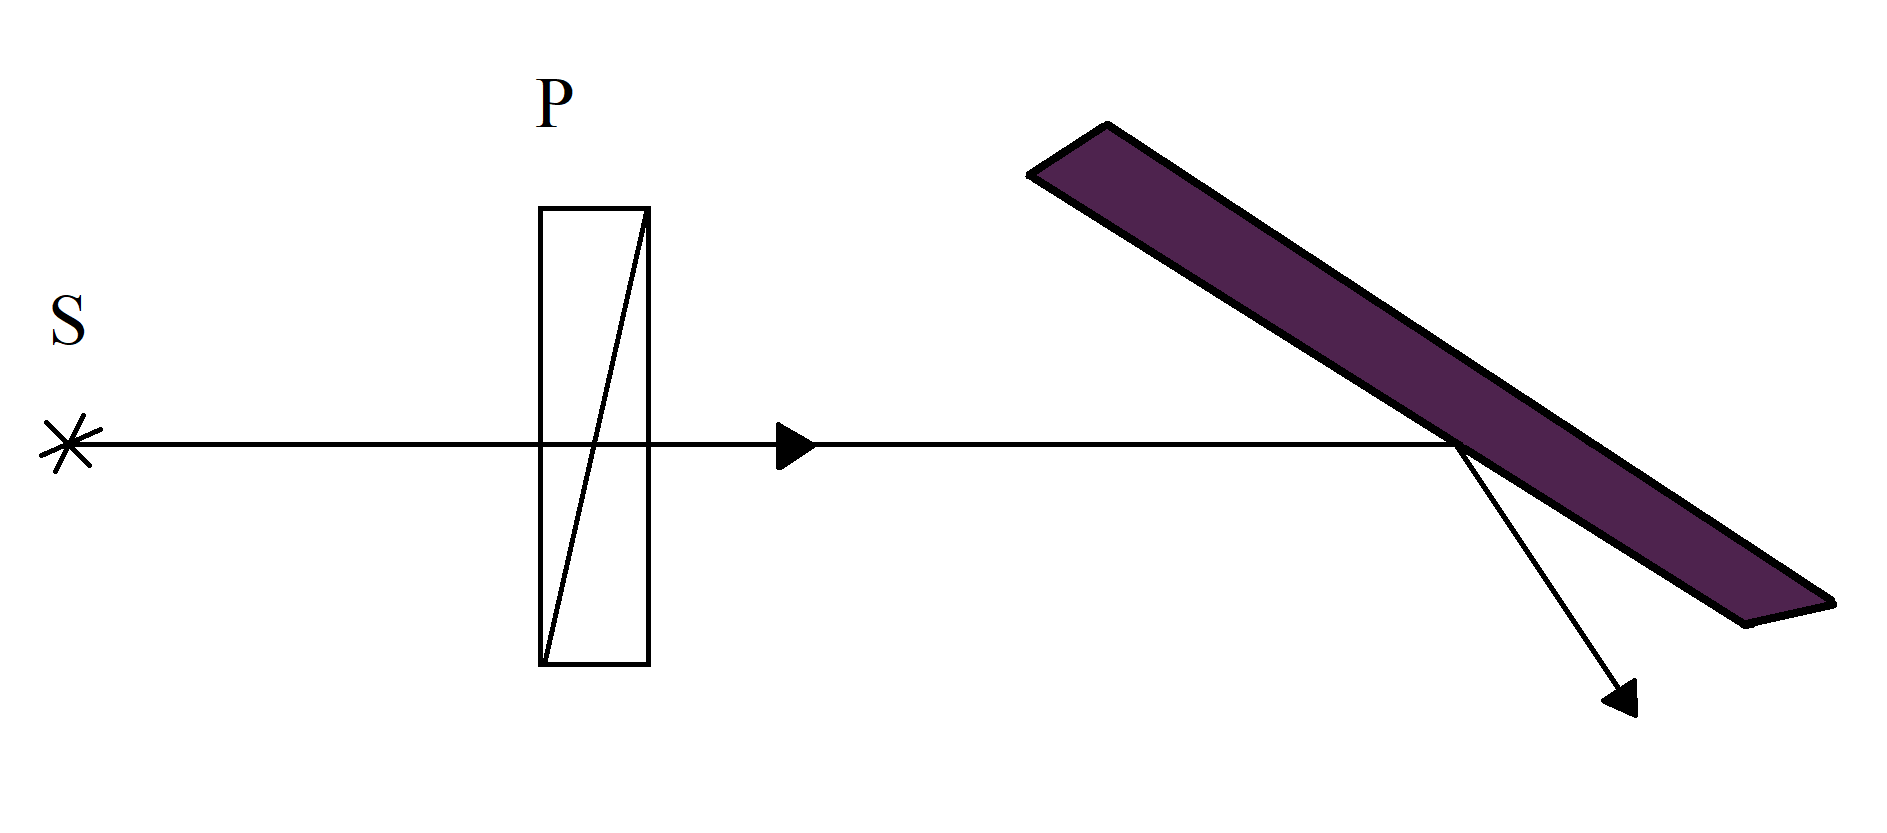
\includegraphics[width=1\textwidth]{images/mirror.png}
    \caption{We put a polaroid P and a mirror (violet one) on the way of light.}
    %\label{fig:}
\end{figure}
\end{minipage}
\hfill
\begin{minipage}{0.35\textwidth}
	Now we can make a rough estimation of polarization direction. And by adding the second polaroid we can also etimate it's polarization direction.
	\begin{align*}
		&P_1 \colon -4^\circ&\\
		&P_2 \colon 291^\circ&
	\end{align*}
\end{minipage}

	\frametitle{The experiment setup}
}
\frame{
\begin{minipage}{0.45\textwidth}
    \begin{figure}[h]
    \centering
    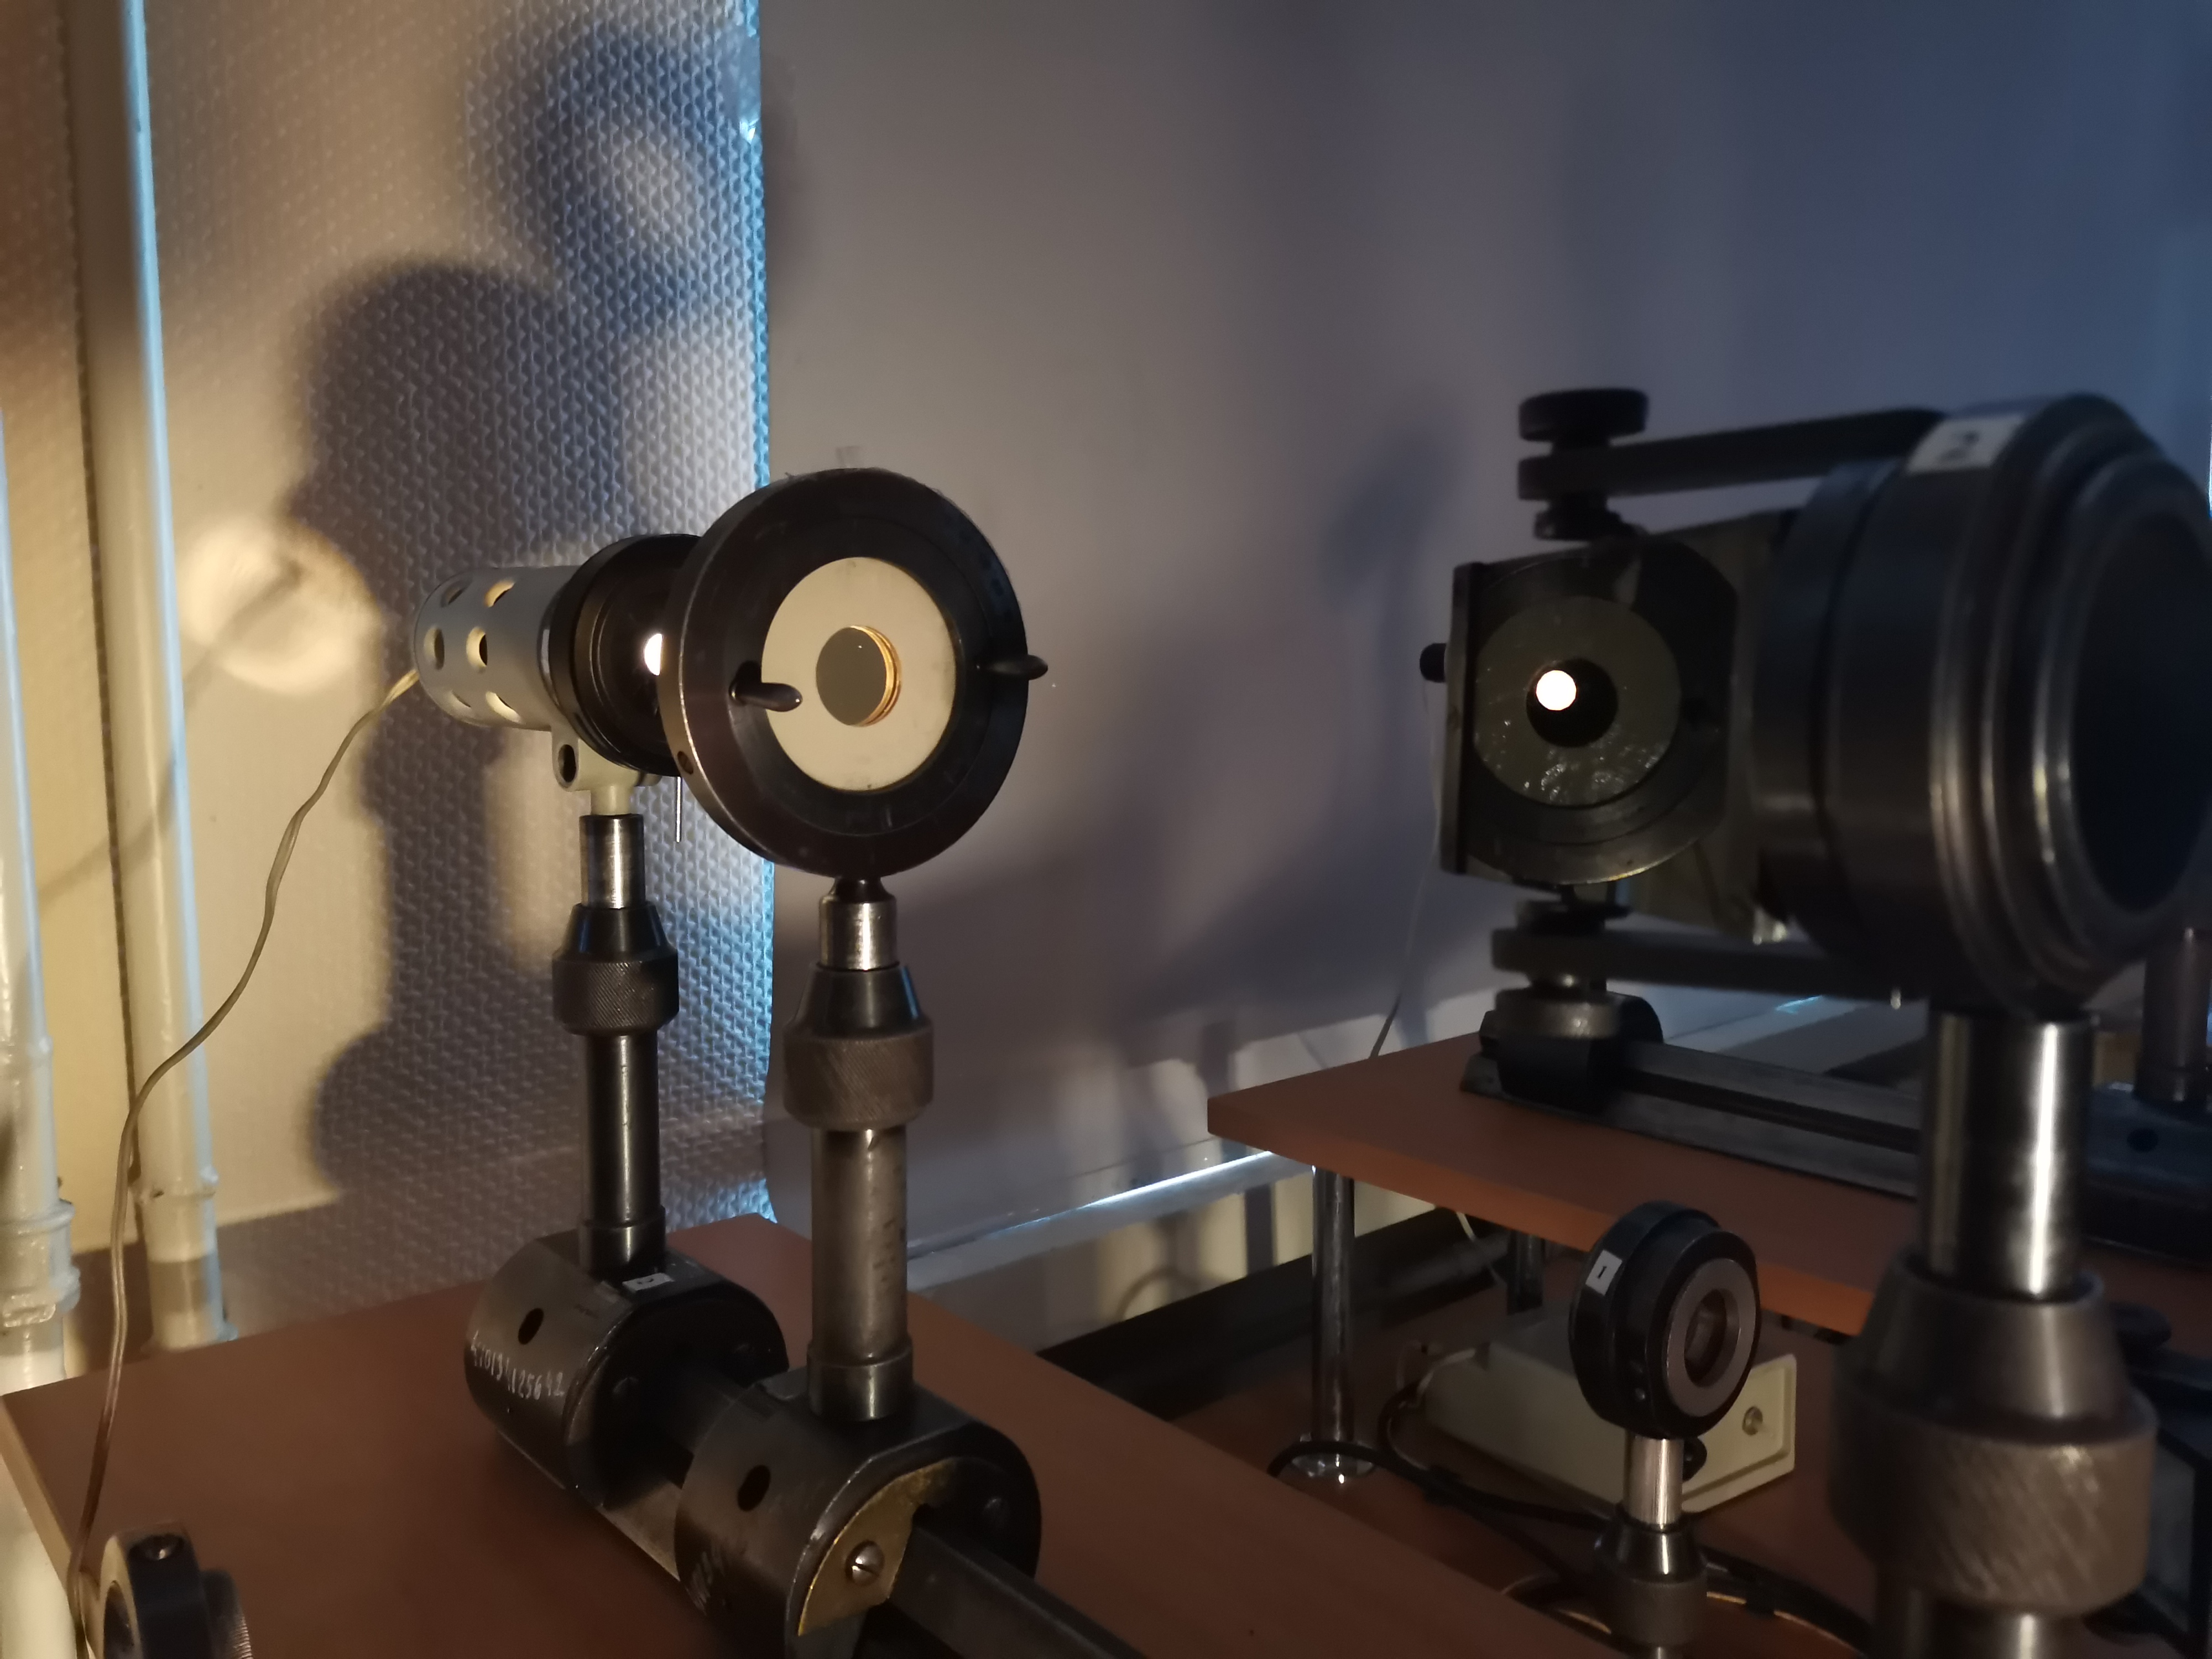
\includegraphics[width=1.1\textwidth]{images/mirror-pol.jpg}
    \caption{With the mirror.}
	\end{figure}
\end{minipage}
\hfill
\begin{minipage}{0.45\textwidth}
    \begin{figure}[h]
    \centering
    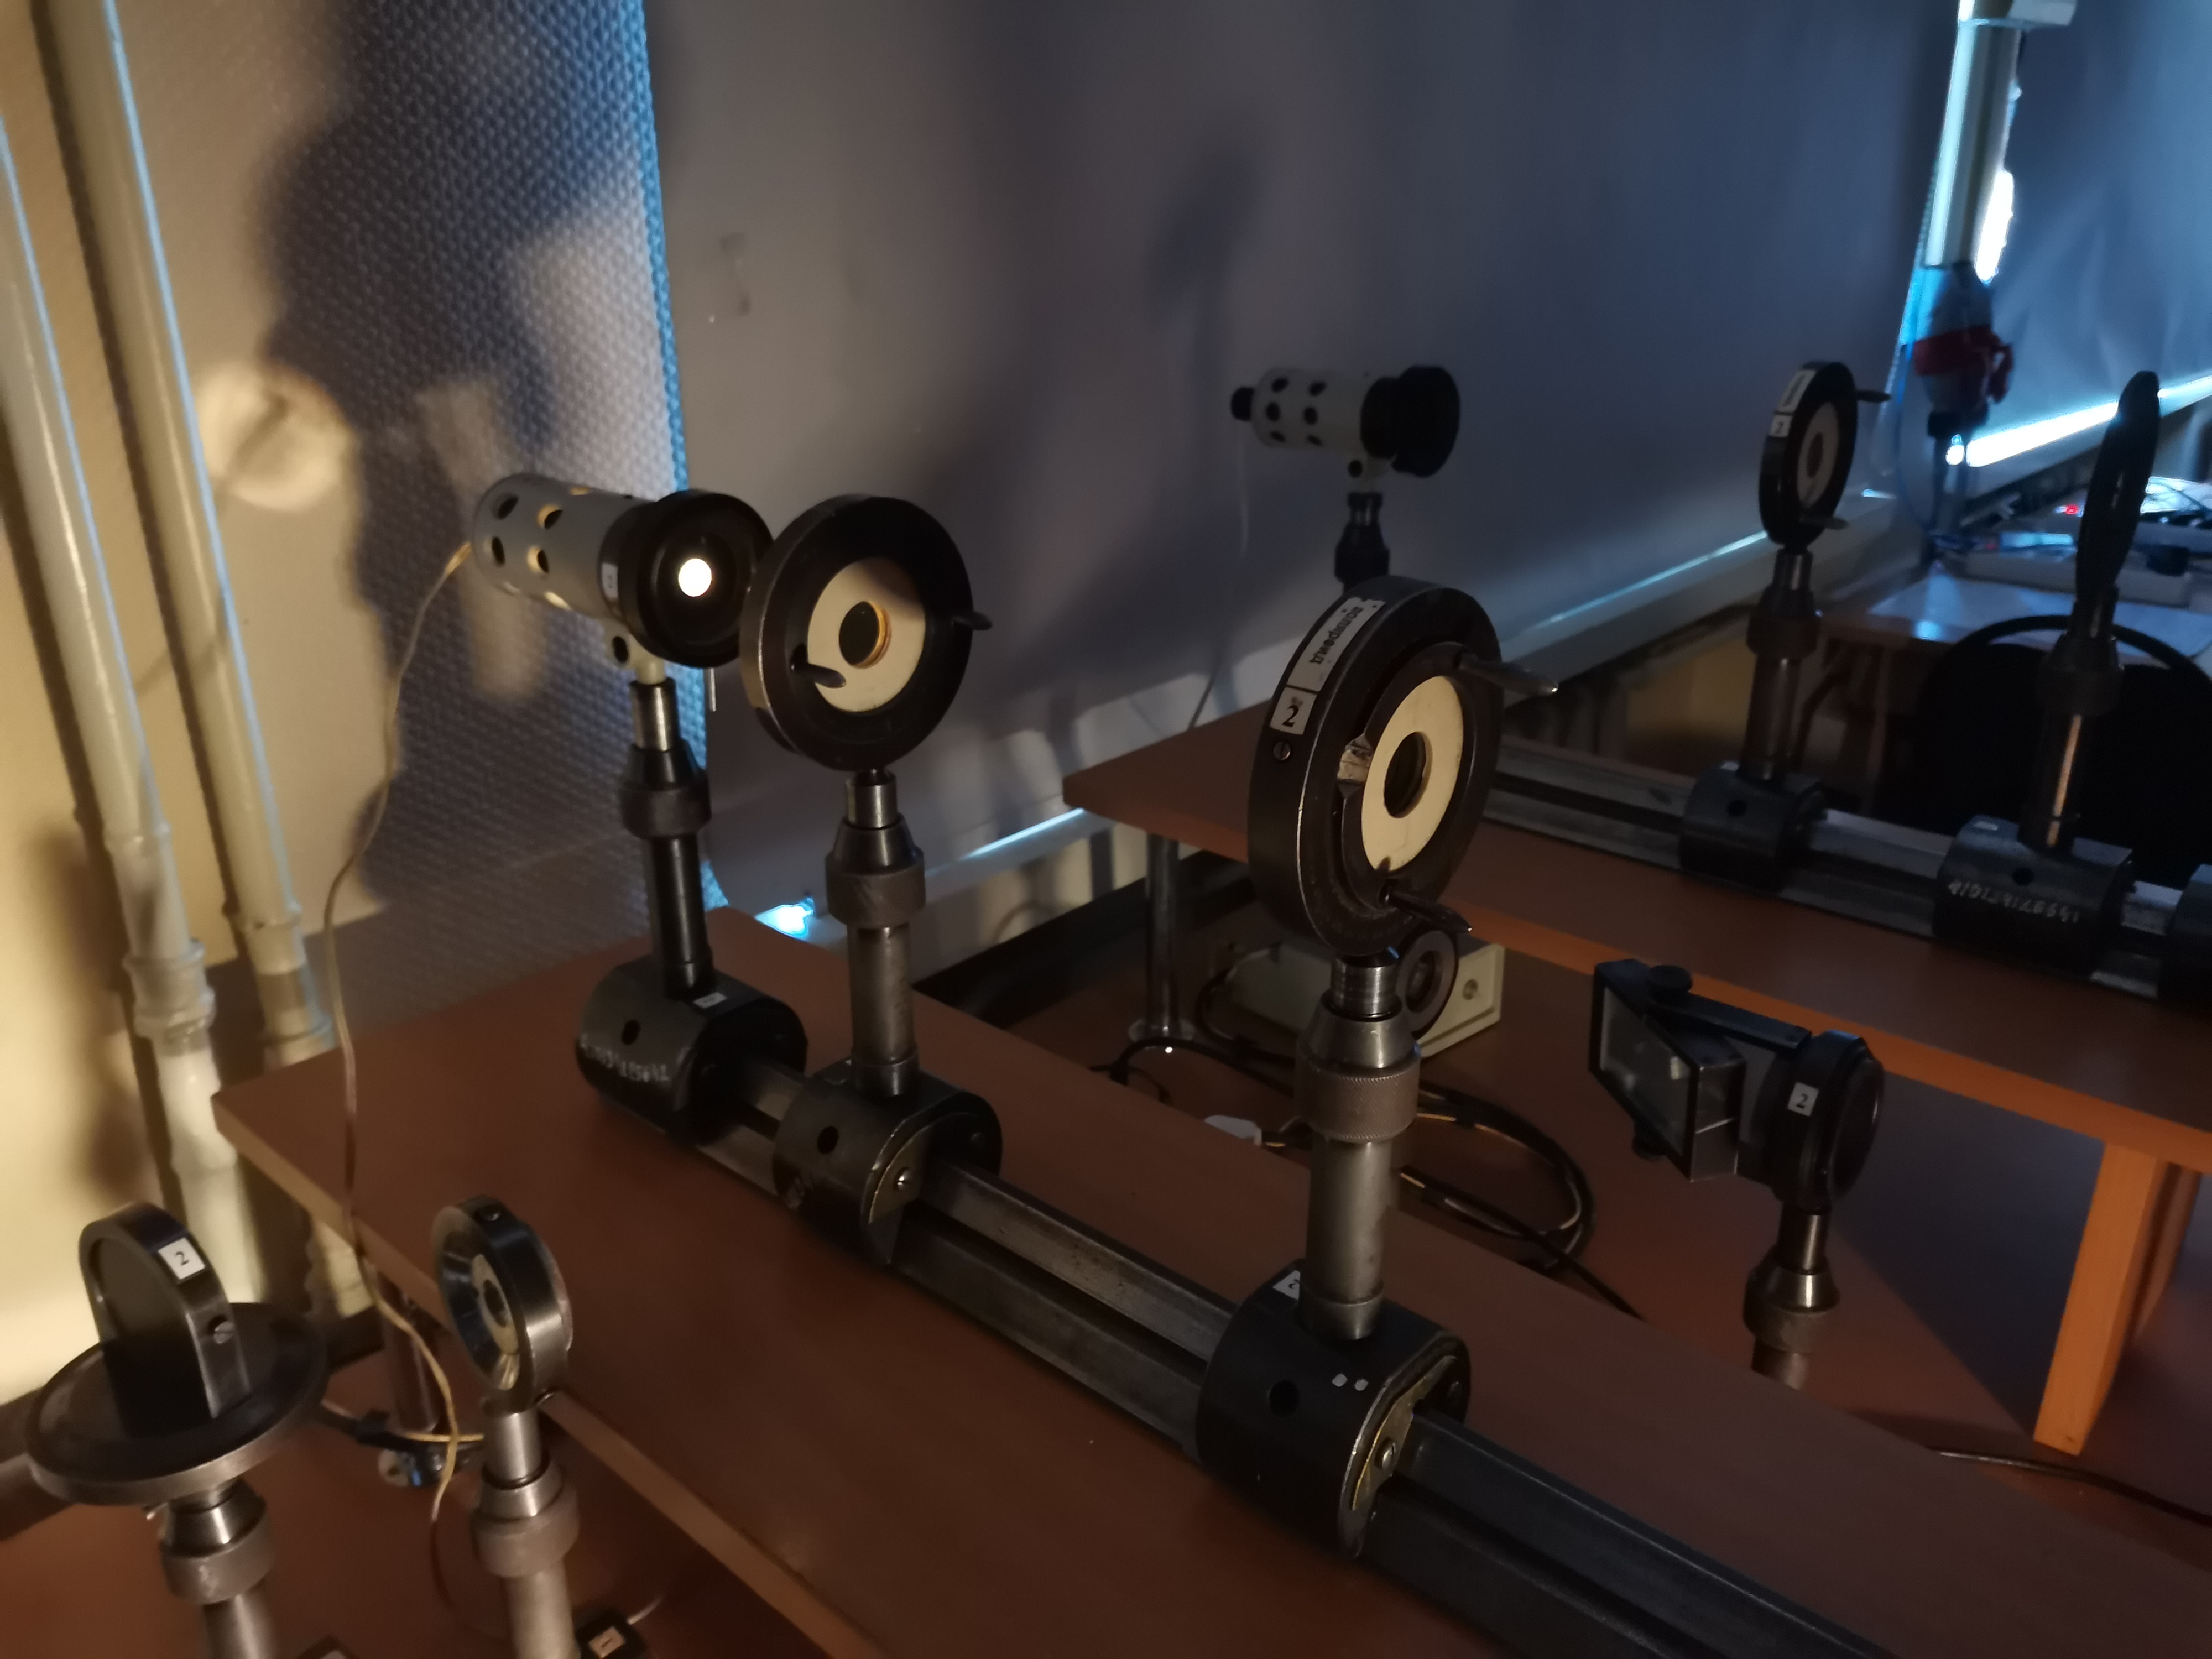
\includegraphics[width=1.1\textwidth]{images/2pol.jpg}
    \caption{The second polaroid.}
	\end{figure}
\end{minipage}
	\frametitle{The experiment photos}
}




\section{Brewester}

\frame{
And God said let there be light, and there was light
\begin{equation}
	\triangle E(\vc{r},t) - \mu_0 \varepsilon(\vc{r}) \frac{\partial^2}{\partial t^2} E(\vc{r}, t) = \mu_0 \frac{\partial^2}{\partial t^2} P_{in}(\vc{r},t)
\end{equation}
Which is solved as
\begin{equation*}
	E(\vc{r},t) = \frac{1}{2} E_0 e^{i(\beta y - \omega t)} + \const
\end{equation*}
And we assume:
\begin{equation*}
	E(\vc{r}, t) = A(t) E(s').
\end{equation*}	\frametitle{Theory behind the phenomenon}
}
\frame{
\begin{minipage}{0.35\textwidth}
    \begin{figure}[h]
    \centering
    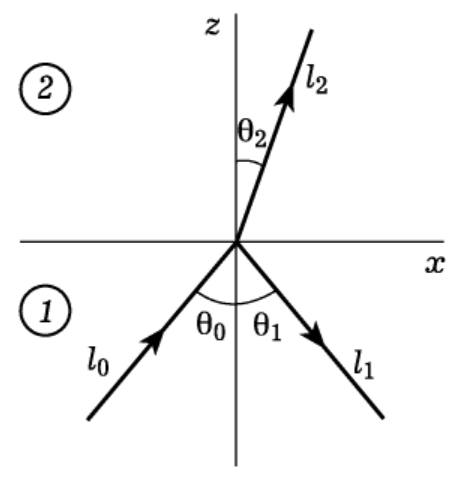
\includegraphics[width=1\textwidth]{images/brust.png}
    \caption{0 stands for a in-going wave, 1 stands for a transmitted wave, 2 stand for a reflected wave.}
    %\label{fig:}
\end{figure}
\end{minipage}
\hfill
\begin{minipage}{0.55\textwidth}
	 An incredible aspect describes the $\theta_p = \theta_0$ wich gives $\theta_0 + \theta_2 = \pi/2$.

	 With this and Snell's law we obtain:
	 \begin{equation}
	 	\tg \theta_p = \sqrt{\frac{\varepsilon_2}{\varepsilon_1}} = n.
	 \end{equation}
	 Where $\theta_p$ is the angle of polarization or \textit{Brewster's angle}.
\end{minipage}

	\frametitle{The main formula}
}
\frame{
\begin{minipage}{0.55\textwidth}
    \begin{figure}[h]
    \centering
    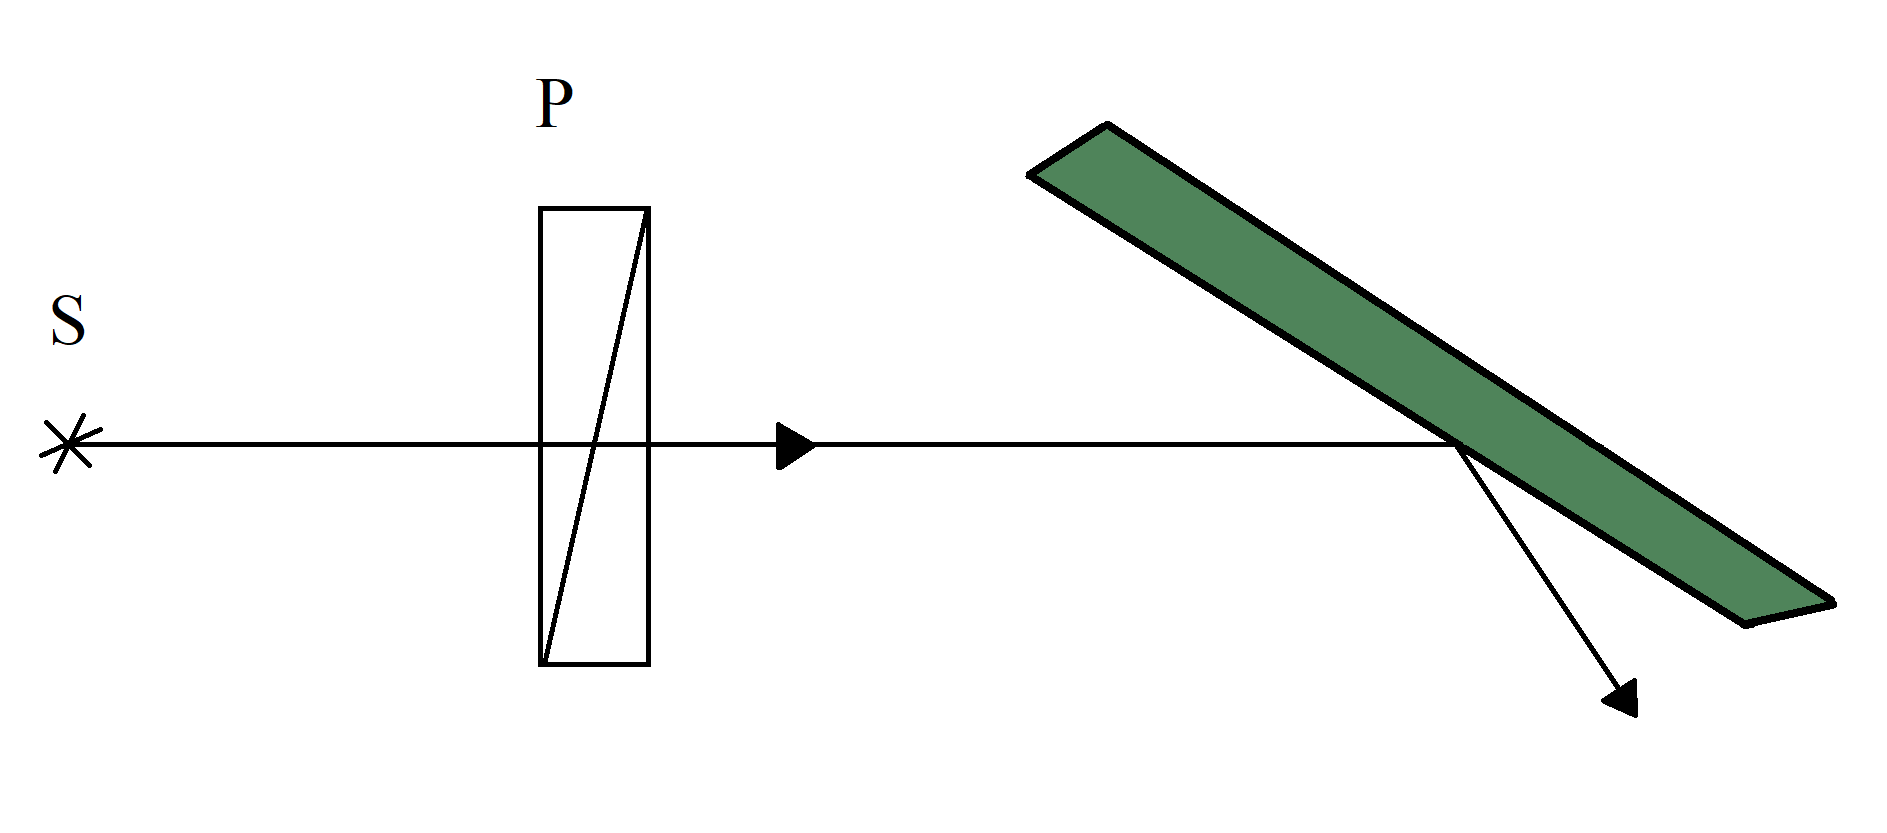
\includegraphics[width=1\textwidth]{images/ebonit.png}
    \caption{By rotating green ebonite plain we obtain several angles.}
    %\label{fig:}
\end{figure}
\end{minipage}
\hfill
\begin{minipage}{0.35\textwidth}
	\begin{center}
	\begin{tabular}{ |c|c|c| } 
		\hline
		name & $\theta_p$ & $\tg(\theta_p)$ \\
 		\hline
 		K & 240 & 1.73 \\ 
 		E & 237 & 1.54 \\ 
 		K & 237 & 1.54 \\ 
 		E & 238 & 1.60 \\ 
 		K & 236 & 1.48 \\ 
 		E & 239 & 1.66 \\ 
 		\hline
	\end{tabular}
	\end{center}
	The measurements were taken apart from each other.
\end{minipage}

	\frametitle{Our measurements}
}
\frame{
For the most beauty we assume that well is 1D, and the equastion:
\begin{equation}
	\frac{d A}{d t} = \frac{1}{2} v_g (\Gamma_{MD}G - i \Gamma_{MD} N_r)A,
\end{equation}
where $v_g = c/n_r$ is the speed of light in vacuum. And $\Gamma_{MD}G = g$ is so called gain coefficient.	\frametitle{Results}
}


\section{Stoletov}

\frame{
\begin{minipage}{0.55\textwidth}
    \begin{figure}[h]
    \centering
    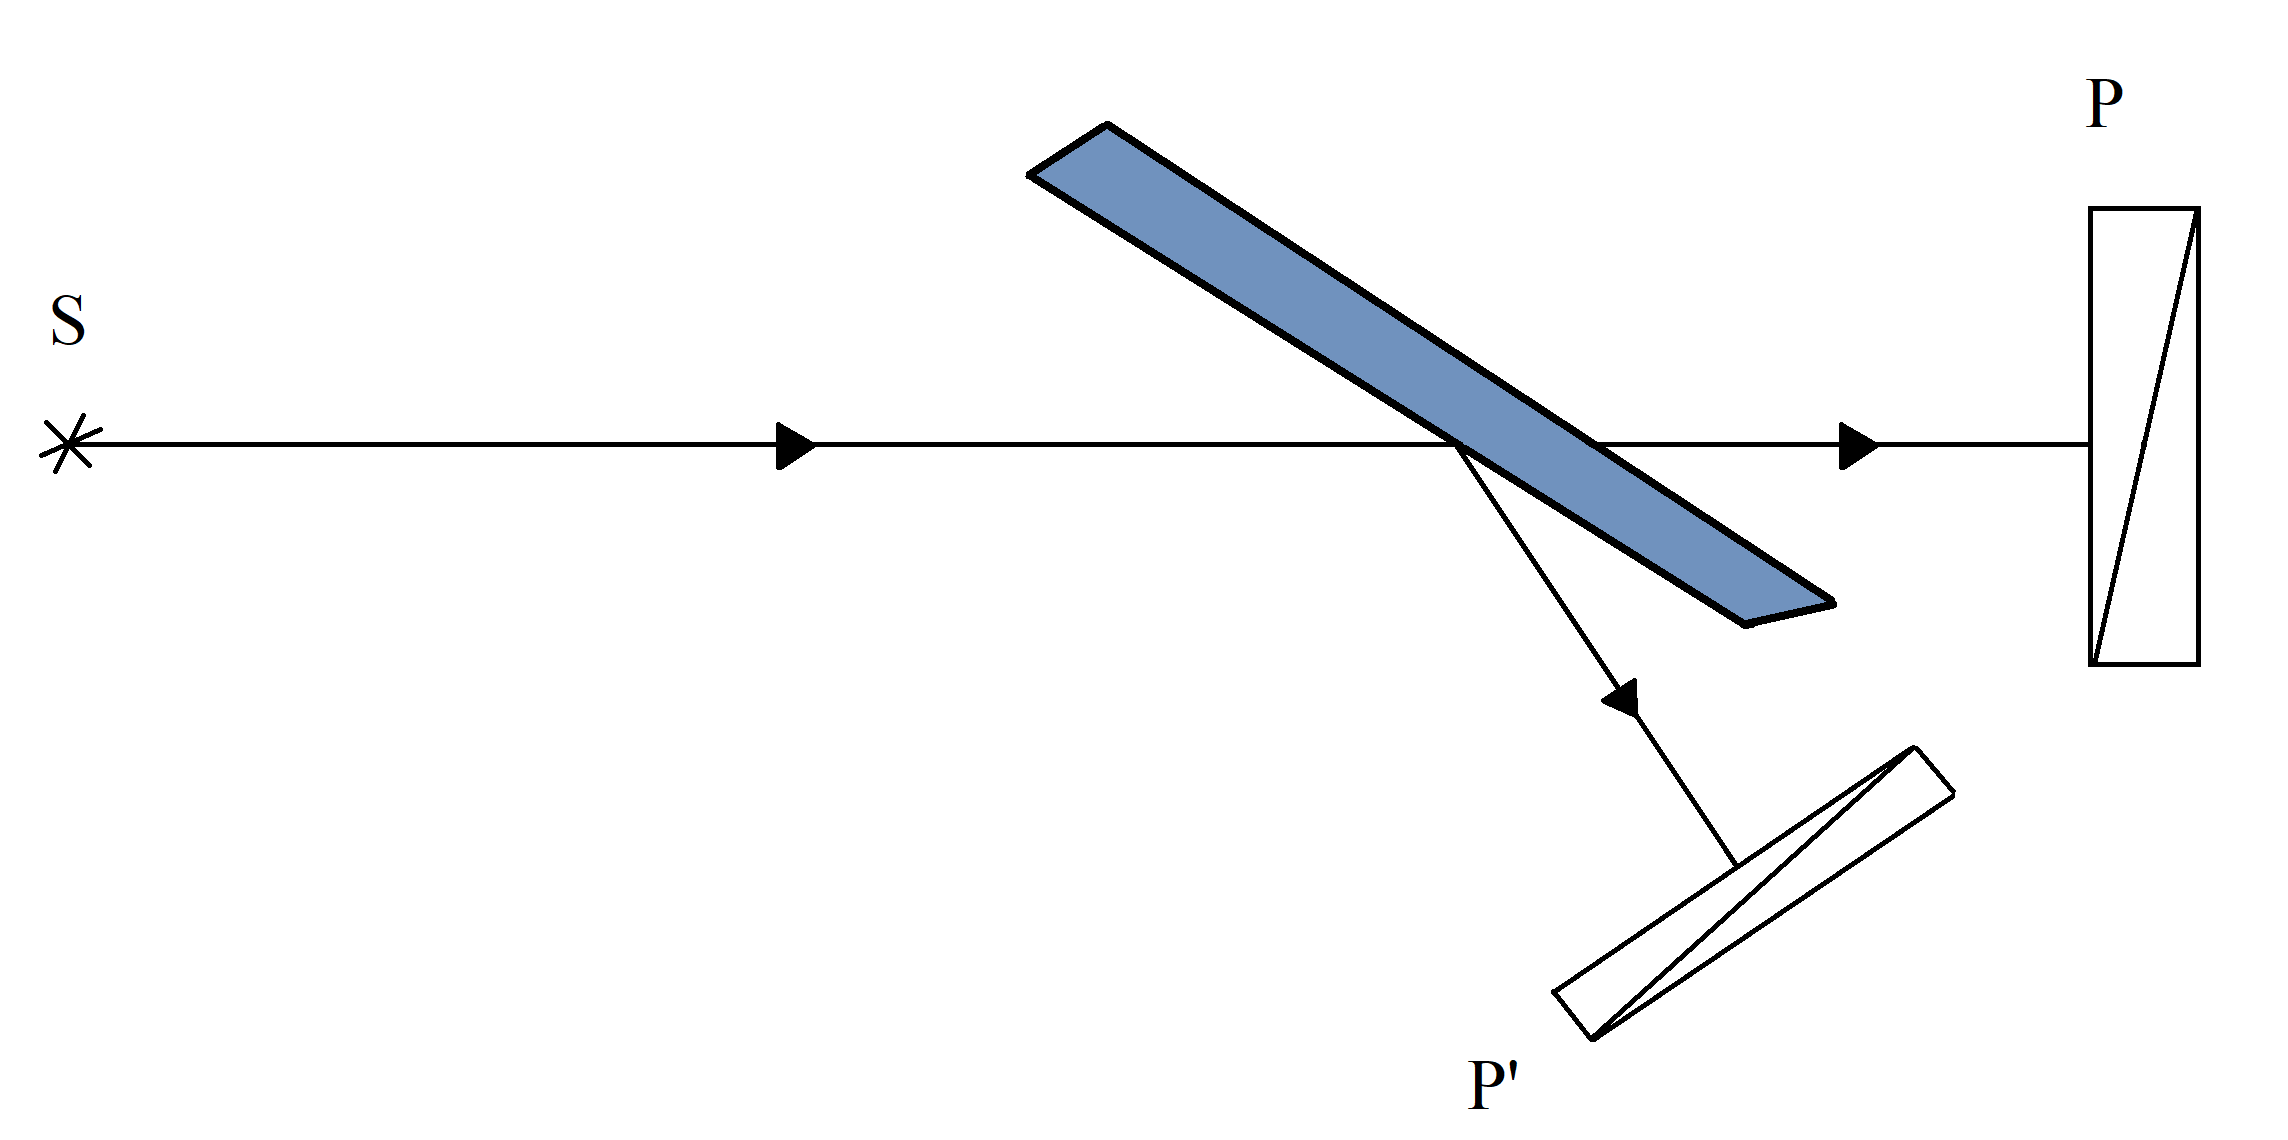
\includegraphics[width=1\textwidth]{images/stoletov.png}
    \caption{The beam goes right to the stack of glass (light blue) and then splits to two polaroids that we investigate before.}
    %\label{fig:}
\end{figure}
\end{minipage}
\hfill
\begin{minipage}{0.35\textwidth}
    Here we have to observe the with the polaroids from previous observation the direction of vector $E$.

    The polaroids were crossed when:
    \begin{align*}
    	P_1 \colon 98^\circ\\
    	P_2 \colon 26^\circ
    \end{align*}    
\end{minipage}
  \frametitle{Observation of reflected and rejected light}
}

\frame{
\begin{minipage}{0.55\textwidth}
    \begin{figure}[h]
    \centering
    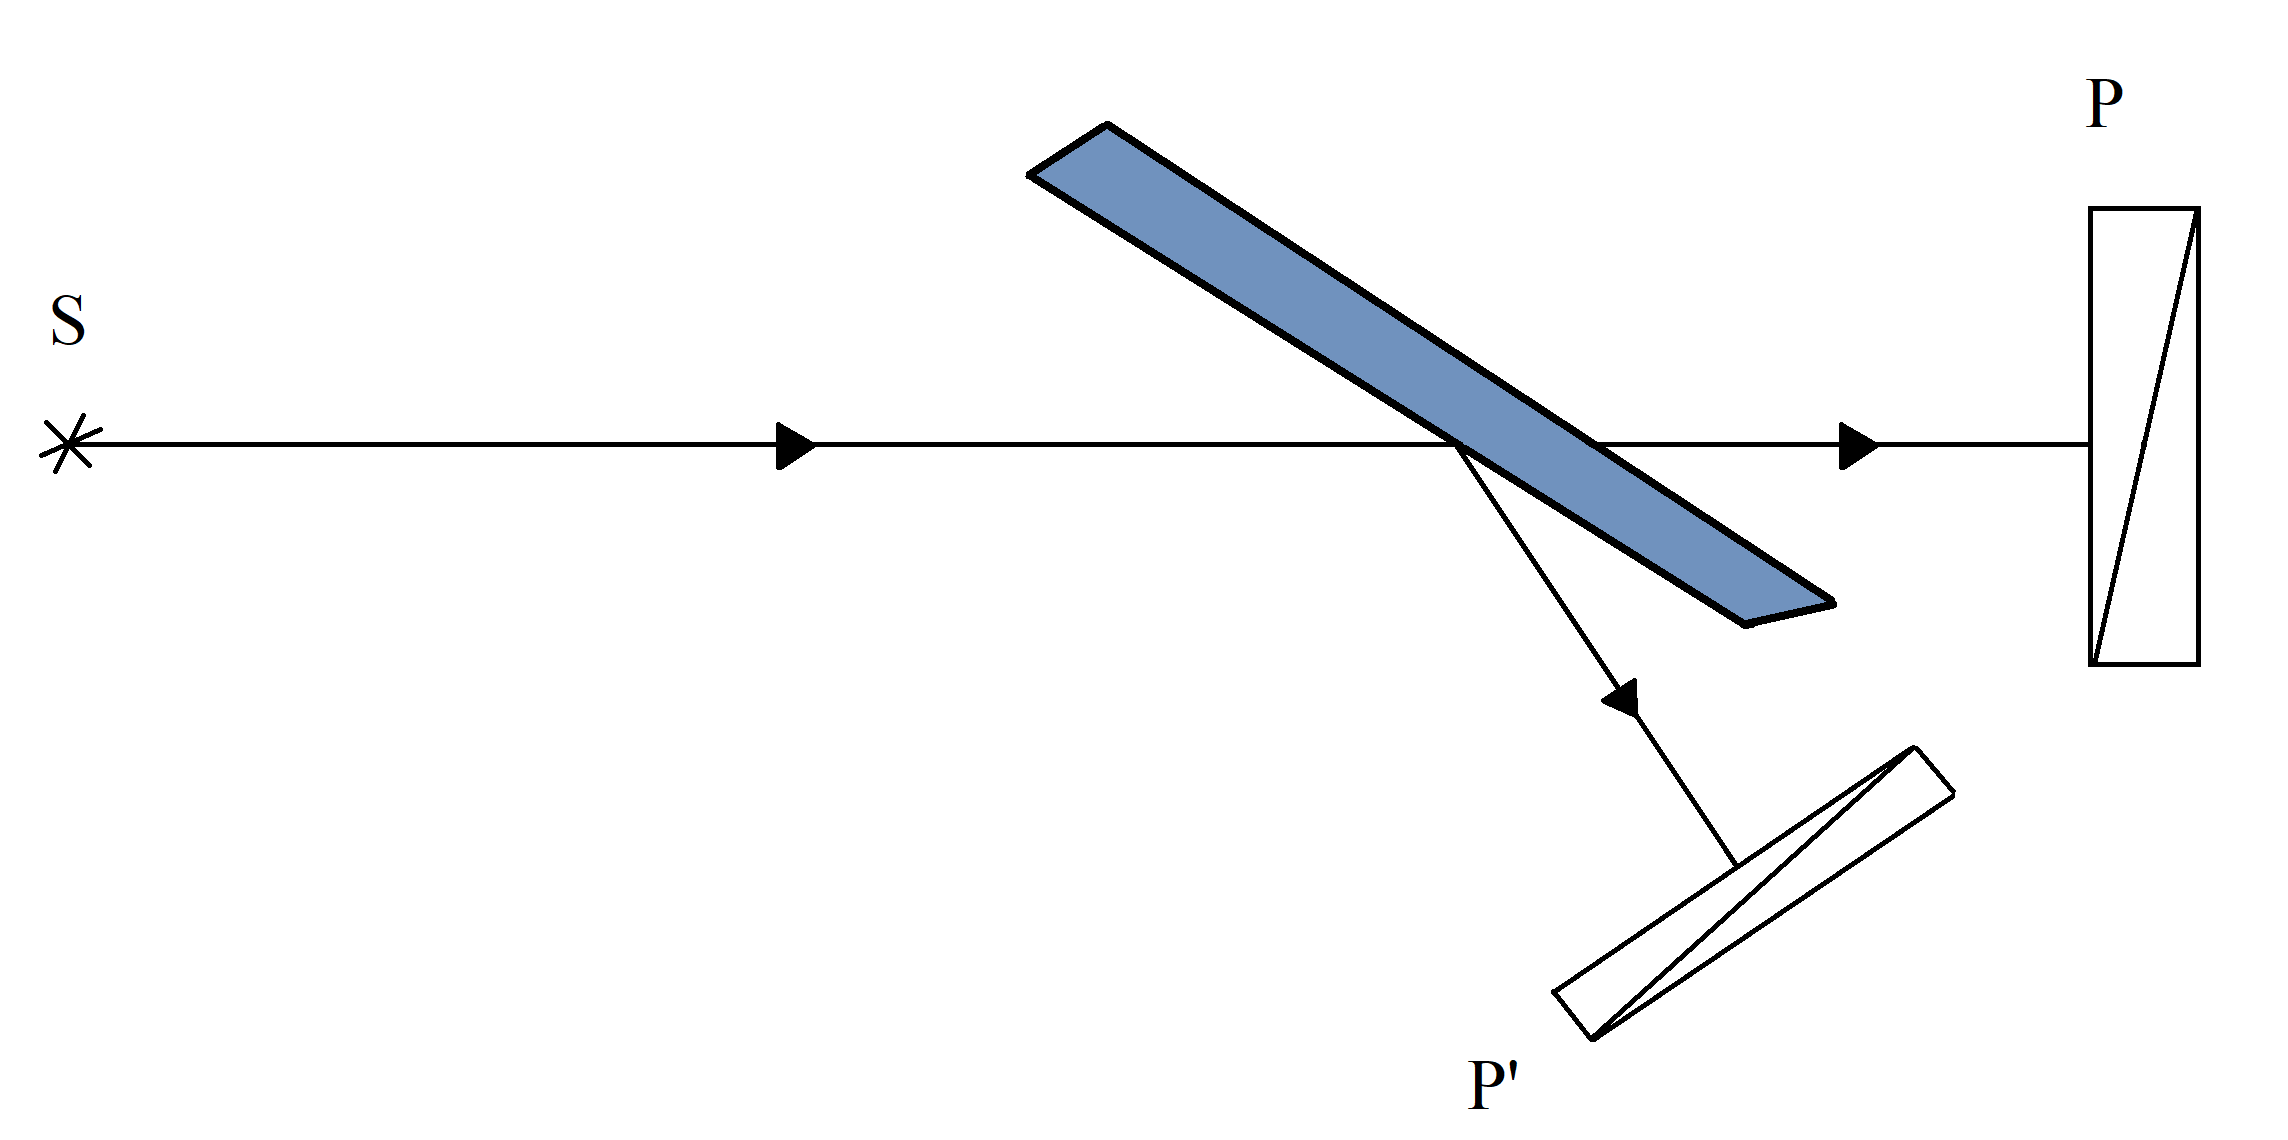
\includegraphics[width=1\textwidth]{images/stoletov.png}
    \caption{The beam goes right to the stack of glass (light blue) and then splits to two polaroids that we investigate before.}
    %\label{fig:}
\end{figure}
\end{minipage}
\hfill
\begin{minipage}{0.35\textwidth}
    So as was expected the reflected and transmitted light had an orthogonal $E$.

    The polaroids are crossed
    \begin{align*}
    	&P_1 \colon 98^\circ&\\
    	&P_2 \colon -265^\circ&
    \end{align*}
\end{minipage}
  \frametitle{Results}
}

\frame{
\begin{minipage}{0.55\textwidth}
    \begin{figure}[h]
    \centering
    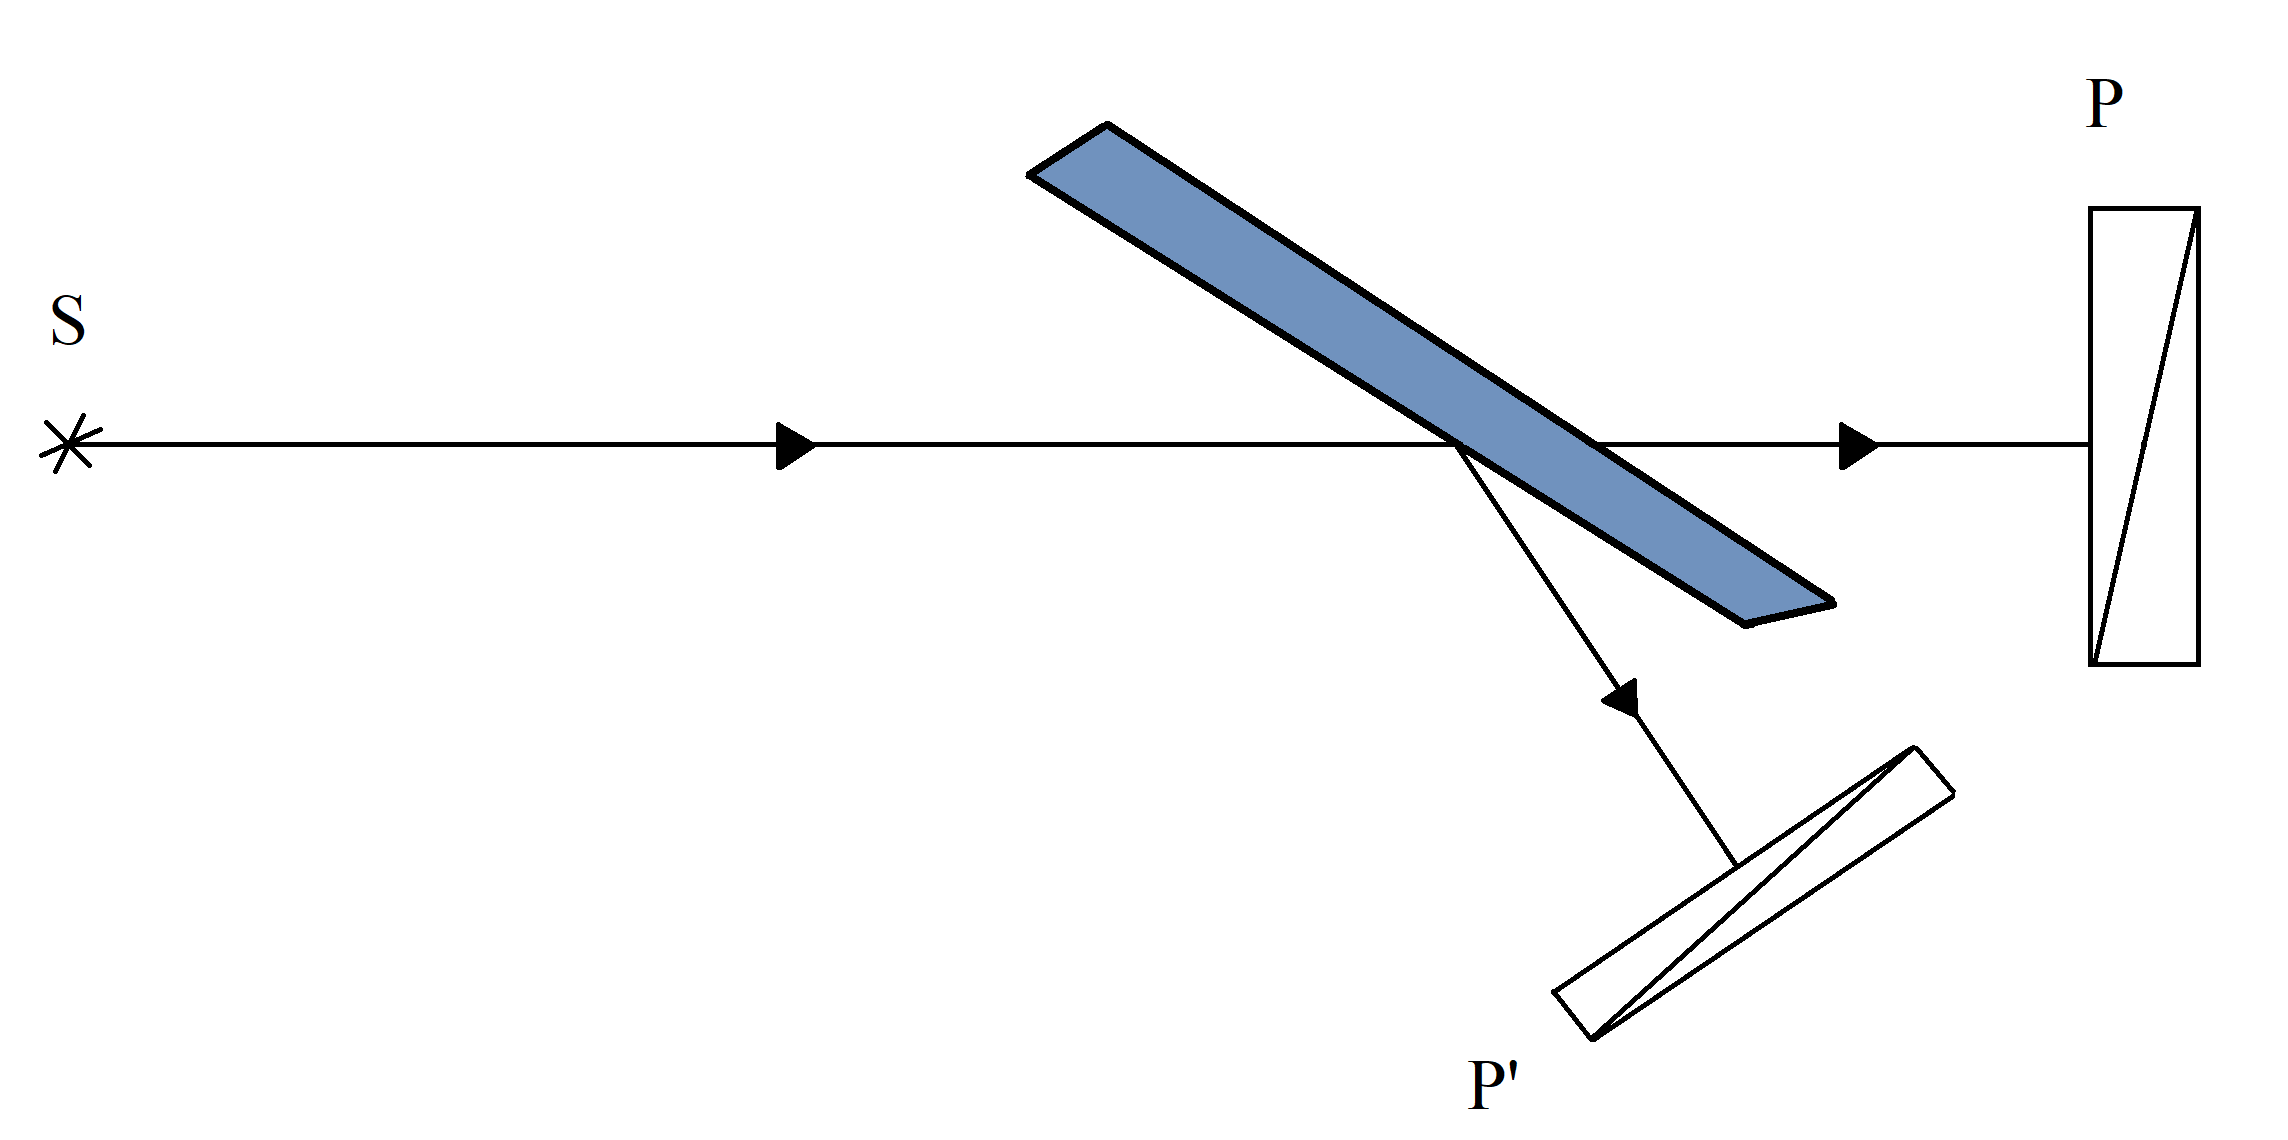
\includegraphics[width=1\textwidth]{images/stoletov.png}
    \caption{The beam goes right to the stack of glass (light blue) and then splits to two polaroids that we investigate before.}
    %\label{fig:}
\end{figure}
\end{minipage}
\hfill
\begin{minipage}{0.35\textwidth}
    Now we synchronize them by adding the period ($2 \pi$):
    \begin{align*}
        P_1 \colon 98^\circ\\
        P_2 \colon 95^\circ
    \end{align*}
    So the polaroids are again synchronized, as we expected it to be for transmitted and reflected light.
\end{minipage}
  \frametitle{Pleasant to look at results}
}


\section{2xRefracting}

\frame{
\begin{minipage}{0.55\textwidth}
    \begin{figure}[h]
    \centering
    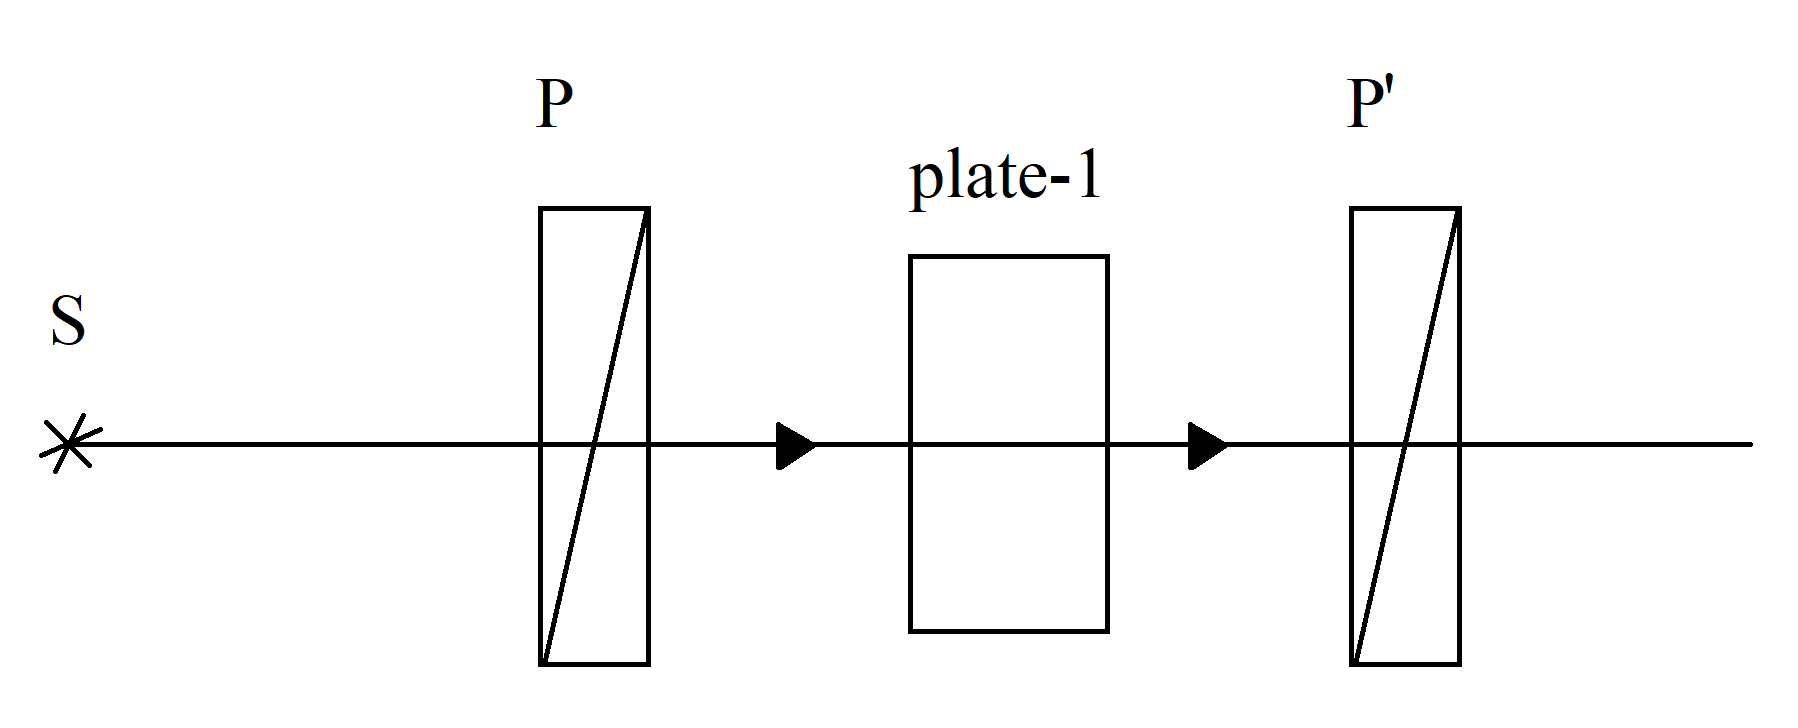
\includegraphics[width=1\textwidth]{images/crystplast.png}
    \caption{We add two crossed polaroids and the double refracting plate between them.}
    %\label{fig:}
\end{figure}
\end{minipage}
\hfill
\begin{minipage}{0.35\textwidth}
    So, when the polarizations match we observe maximum, and otherwise minimum of intensity.
    \begin{align*}
        \text{max} \colon 227^\circ\\
        \text{min} \colon 275^\circ
    \end{align*}
\end{minipage}
  \frametitle{Experimental set up 1}
}

\frame{
\begin{minipage}{0.55\textwidth}
    \begin{figure}[h]
    \centering
    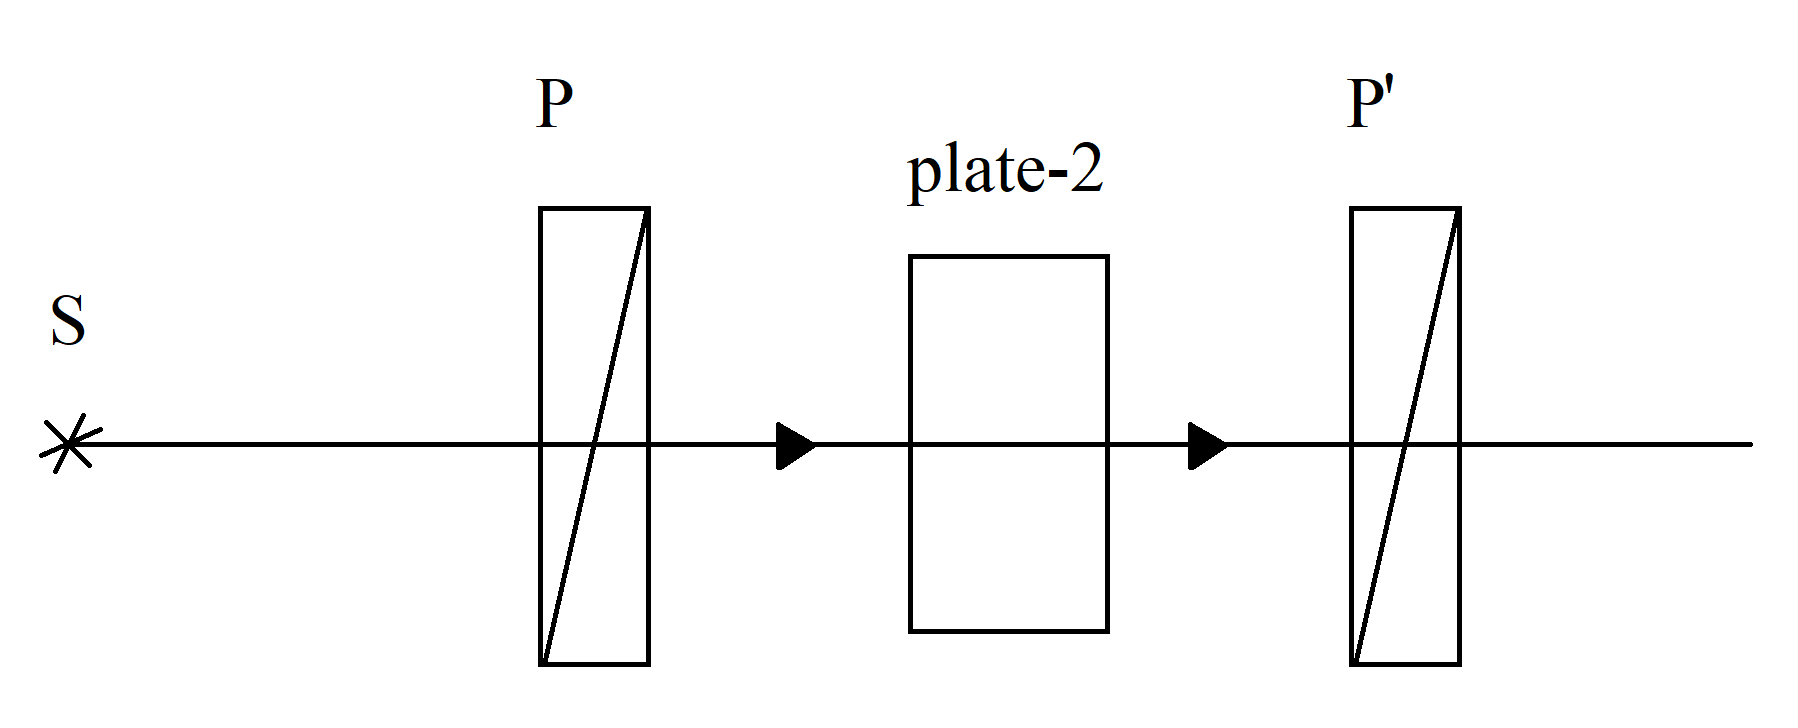
\includegraphics[width=1\textwidth]{images/crystplast2.png}
    \caption{We add two crossed polaroids and the double refracting plate between them.}
    %\label{fig:}
\end{figure}
\end{minipage}
\hfill
\begin{minipage}{0.35\textwidth}
    So, when the polarizations match we observe maximum, and otherwise minimum of intensity.
    \begin{align*}
        \text{max} \colon 86^\circ\\
        \text{min} \colon 43^\circ
    \end{align*}
\end{minipage}
  \frametitle{Experimental set up 2}
}


\section{Lambda}

\frame{
\begin{minipage}{0.35\textwidth}
    \begin{figure}[h]
    \centering
    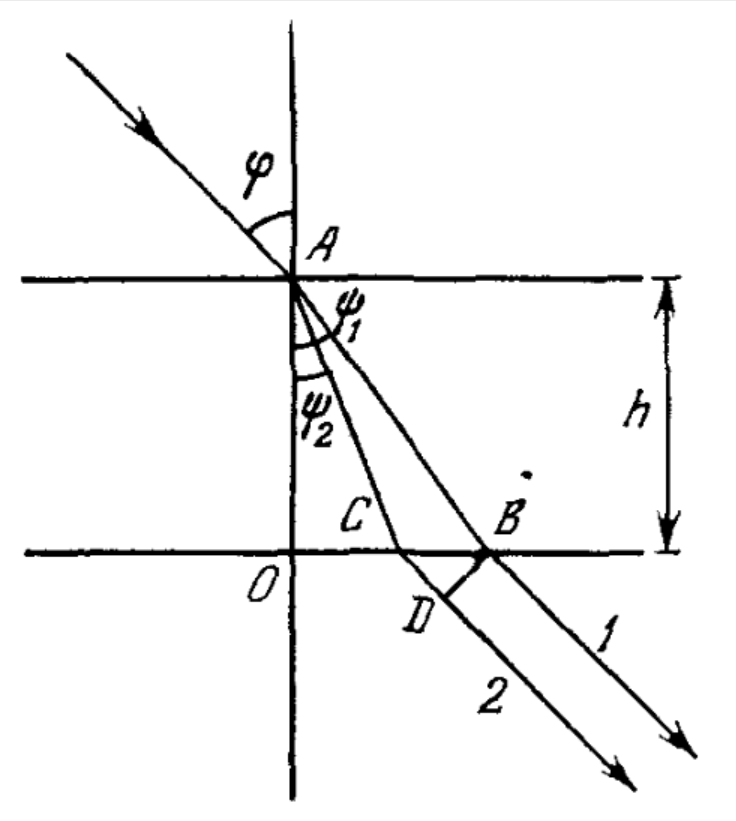
\includegraphics[width=1\textwidth]{images/intercolor.png}
    \caption{The crystal refract the beam differently.}
    %\label{fig:}
\end{figure}
\end{minipage}
\hfill
\begin{minipage}{0.55\textwidth}
    Going through the crystal plate the light gains the phase difference of
    \begin{equation*}
    	\Delta = h (n_2 \cos \psi_2 - n_1 \cos \psi_1),
    \end{equation*}
    for different refraction coefficient and refracting angles that have a small difference, so
    \begin{equation*}
    	\Delta = h \cos \psi (n_2 - n_1).
    \end{equation*}
\end{minipage}
  \frametitle{The crystal plate}
}

\frame{
\begin{minipage}{0.55\textwidth}
    \begin{figure}[h]
    \centering
    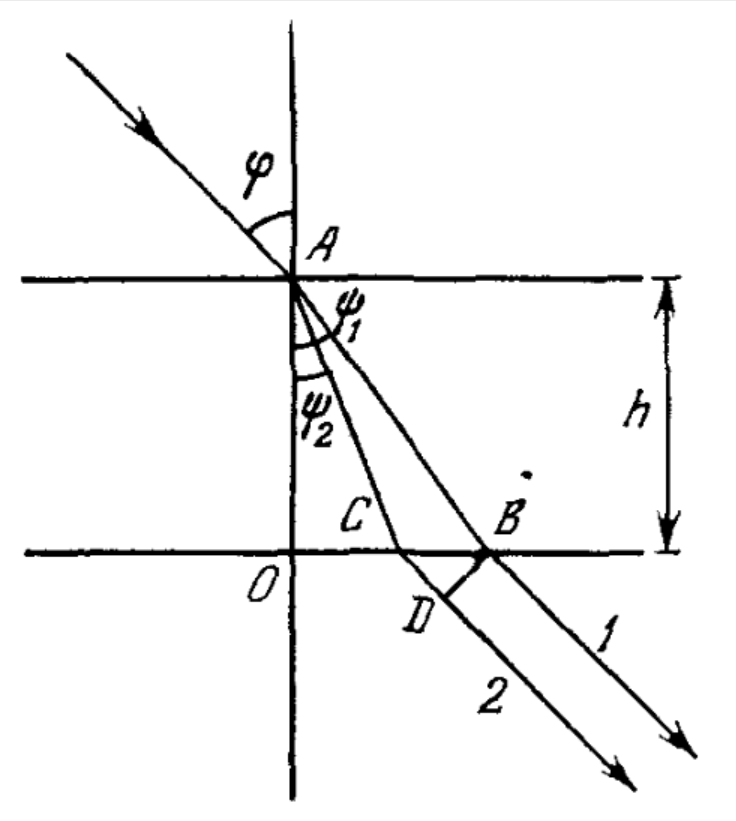
\includegraphics[width=0.7\textwidth]{images/intercolor.png}
    \caption{The setup to get an inreferencion of polarized light that is similar to what we had.}
    %\label{fig:}
\end{figure}
\end{minipage}
\hfill
\begin{minipage}{0.35\textwidth}
    We obtain that the key role plays the wavelength of the light
    \begin{equation*}
        \Delta \varphi = 2 \pi \frac{\Delta}{\lambda}.
    \end{equation*}
    So we will differ the plates (K) regarding to relation of its $\Delta$ to $\lambda$.
\end{minipage}
  \frametitle{After interferencion}
}

\frame{
\begin{minipage}{0.55\textwidth}
    \begin{figure}[h]
    \centering
    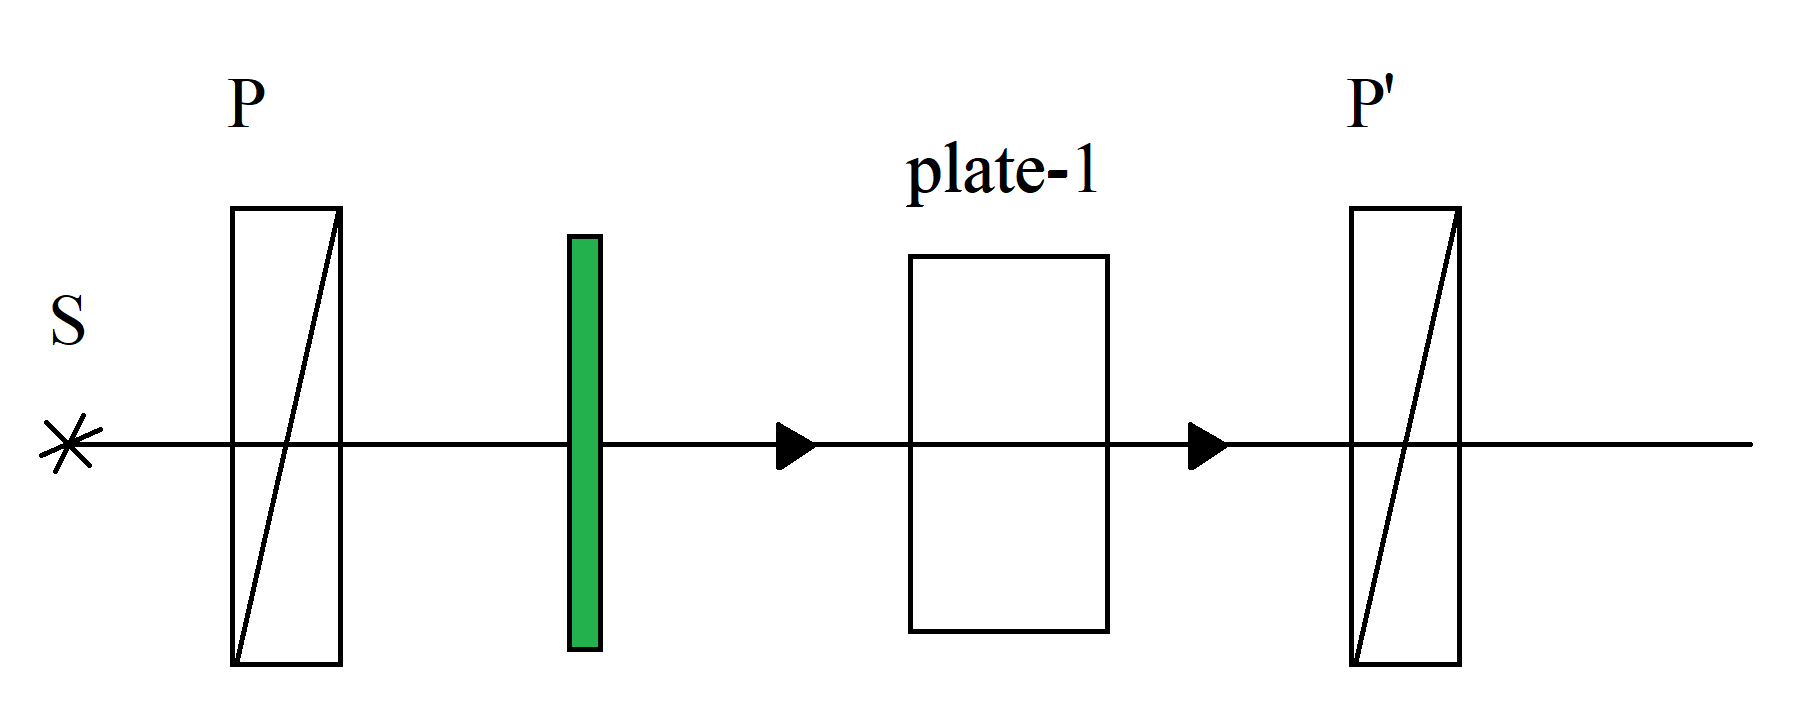
\includegraphics[width=1\textwidth]{images/greeeeeen.png}
    \caption{To the previous setup we add a green light-filter. And rotate the first polaraid so it is horizontal and the plate is  angled as $45^\circ$.}
    %\label{fig:}
\end{figure}
\end{minipage}
\hfill
\begin{minipage}{0.35\textwidth}
    By rotating the polaroid we obtain that plate-1 is $\lambda/4$, because it does not change the intensity, but it changes its polarization and creates phase difference $\pi/2$.
\end{minipage}
  \frametitle{Finding $\lambda/4$}
}
% жирная гифка
% \frame{
% \begin{minipage}{0.18\textwidth}
    \begin{figure}[h]
    \flushleft
    \vspace{-5mm}
    \animategraphics[loop,controls=play,width=0.9\textwidth]{20}{gifs/g1/}{1}{229} 
    \end{figure}
\end{minipage}
\hfill
\begin{minipage}{0.8\textwidth}
We measured all the colors received by the system.
    \begin{figure}[h]
        \centering
        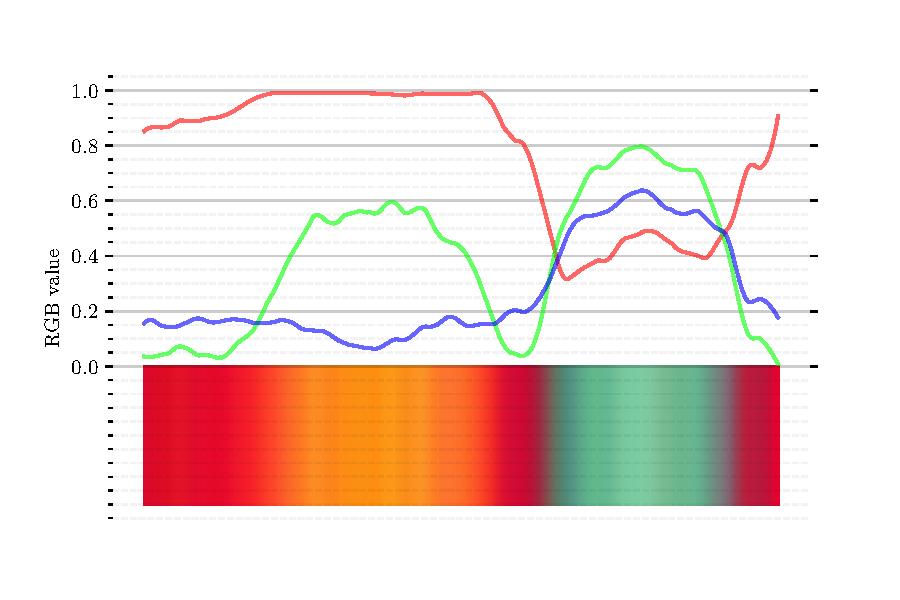
\includegraphics[width=1.1\textwidth]{figures/P1.pdf}
        \vspace{-14mm}
        \caption{Observed colors and RGB decomposition}
    \end{figure}
\end{minipage} \frametitle{RGB measurement}}

\frame{
\begin{minipage}{0.55\textwidth}
    \begin{figure}[h]
    \centering
    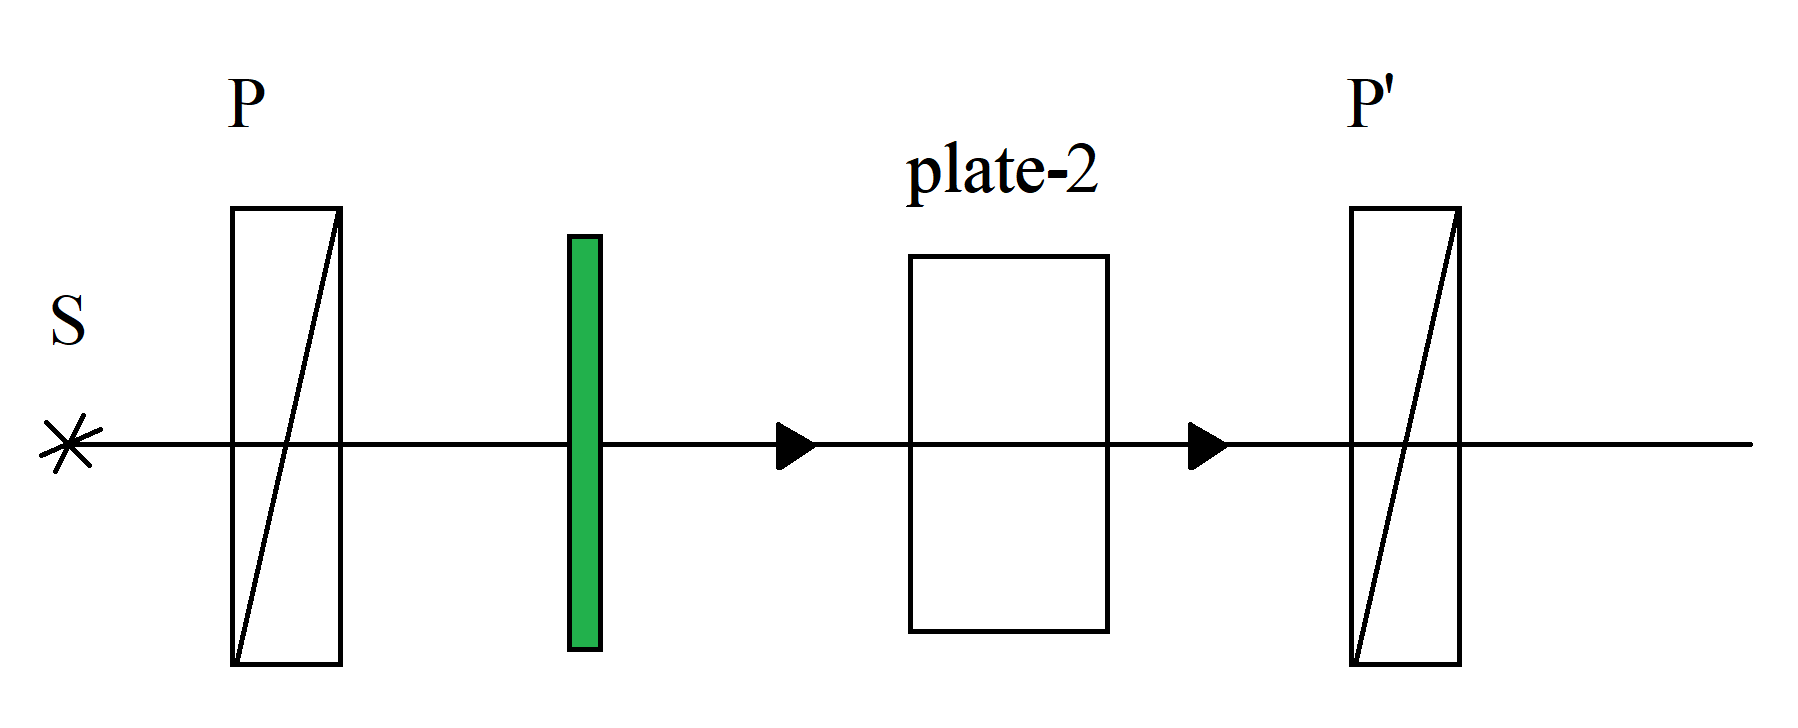
\includegraphics[width=1\textwidth]{images/greeeeeen2.png}
    \caption{To the previous setup we add a green light-filter. And rotate the first polaraid so it is horizontal and the plate is  angled as $45^\circ$.}
    %\label{fig:}
\end{figure}
\end{minipage}
\hfill
\begin{minipage}{0.35\textwidth}
    By rotating the polaroid we obtain that plate-2 is $\lambda/2$, due to observing just fluctuating of its intensity. So no color changing here, no magical video then.
\end{minipage}  \frametitle{Finding $\lambda/2$}
}

\section{Arrow}

\frame{
\begin{minipage}{0.55\textwidth}
    \begin{figure}[h]
    \centering
    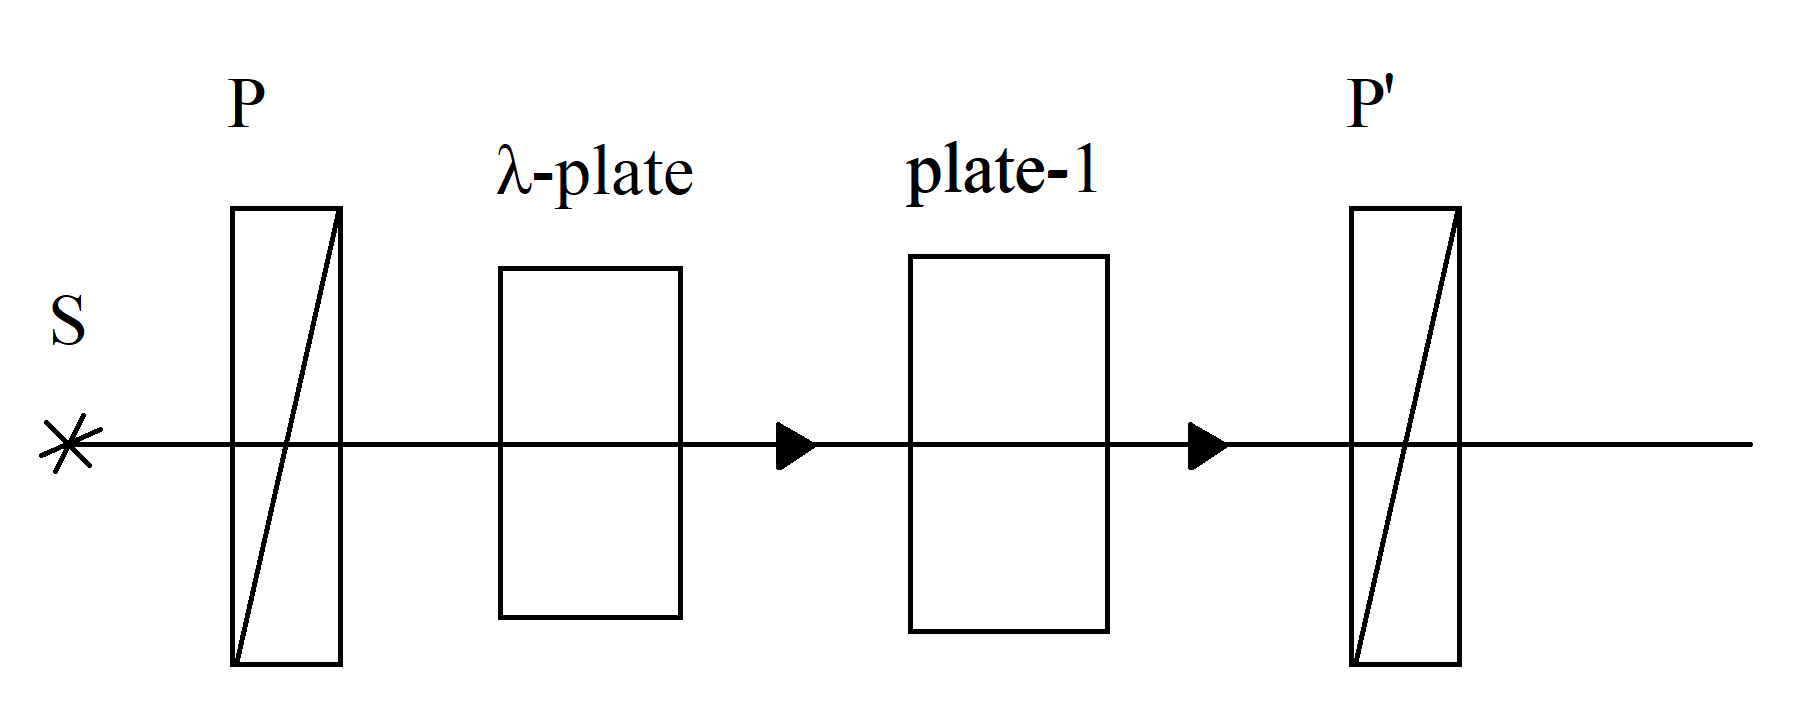
\includegraphics[width=1\textwidth]{images/arrow.png}
    \caption{Now we remove green light-filter and add a plate with the arrow on it.}
    %\label{fig:}
\end{figure}
\end{minipage}
\hfill
\begin{minipage}{0.35\textwidth}
    \begin{itemize}
    	\item with green filter and only arrow between we see no result in previous experiment.
    	\item removing the filter with crossed polaroids we see that the arrow is purple.
    \end{itemize}
\end{minipage}  \frametitle{Adding $\lambda$-plate}
}
\frame{
\begin{minipage}{0.55\textwidth}
    
\end{minipage}
\hfill
\begin{minipage}{0.35\textwidth}
    \begin{itemize}
    	\item 
    \end{itemize}
\end{minipage}  \frametitle{$\Gamma N \Phi K A$}
}


\section{Mica}

% Очень жирная гифка
% \frame{
% % Аналогичным образом сняли цветовую гамму для решетки
The same way we observe color gamma to the grid:

(due to small size of objects we had to detect grid coordinats)

\begin{figure}[h]
\centering
% \vspace{-5mm}
\animategraphics[loop,controls,width=0.9\textwidth]{10}{gifs/g4/}{1}{123} 
\end{figure} \frametitle{RGB measurement}}

\frame{
The study of the interference of polarized light was carried out on a mosaic mica plate.

\phantom{42}

\begin{minipage}{0.55\textwidth}
Phase shift in each cell:
    \begin{center}
	\begin{tabular}{ |c|c|c| } 
		\hline
        % \color{green}
		$3\lambda/4$ & $\lambda/2$ & $3\lambda/4$ \\
		\hline
		$\lambda/4$ & 0 & $\lambda/4$ \\
 		\hline
 		$\lambda$ & $3\lambda/4$ & $\lambda$ \\
 		\hline
	\end{tabular}
	\end{center}
\end{minipage}
\hfill
\begin{minipage}{0.4\textwidth}

\begin{figure}[h]
    \centering
    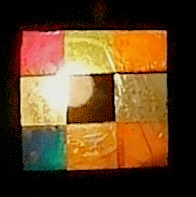
\includegraphics[width=0.75\textwidth]{figures/mica.jpg}
    \caption{Mica plate photo.}
    %\label{fig:}
\end{figure}

    
\end{minipage}

\phantom{42}

The rotation is observed by period $\pi/4$, as expected, with the coincidence of the main directions with the permitted areas of the oscillations of polaroids.  \frametitle{Investigating the cells}
}